\documentclass[../../main.tex]{subfiles}
\graphicspath{{\subfix{../../images/}}}

\begin{document}

    \subsection{Warstwa użytkownika - frontend}

    \subsubsection{Struktura plików}
    Warstwa użytkownika została zaimplementowana przy pomocy frameworku Angular\cite{angular} opartego o język TypeScript (TS). Strukturę plików przedstawia Rysunek \ref{fig:frontend-repo-structure}.

    \begin{figure}[ht!]
        \begin{subfigure}{.5\textwidth}
            \centering
            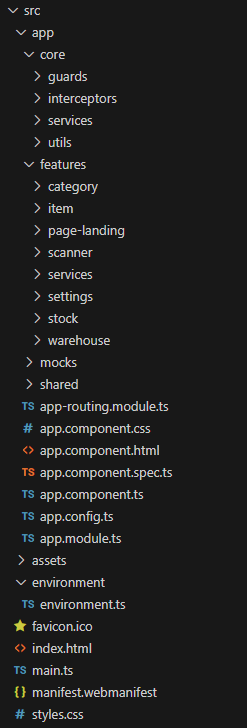
\includegraphics[height=0.4\pdfpageheight]{images/front-repo-structure.png}
            \caption{Ogólna struktura plików}
            \label{fig:front-repo-structure-general}
        \end{subfigure}
        \begin{subfigure}{.5\textwidth}
            \centering
            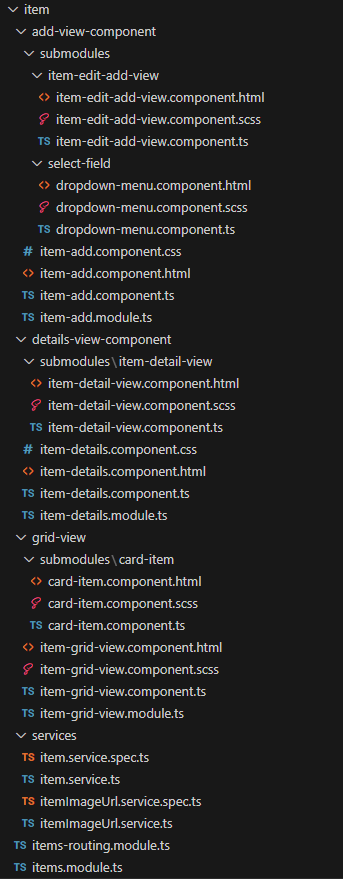
\includegraphics[height=0.4\pdfpageheight]{images/frontend-repo-structure-feature.png}
            \caption{Dokładna struktura jednego z komponentów}
            \label{fig:front-repo-structure-feature}
        \end{subfigure}
        \caption{Struktura plików frontendu}
        \label{fig:frontend-repo-structure}
    \end{figure}

    Aplikacja jest tworzona przy pomocy komponentów. Każdy komponent składa się ze skryptu TS, pliku stylu SCSS oraz pliku układu HTML. Dodatkowo niektóre komponenty korzystają z serwisów napisanych w języku TypeScript. Komponenty graficzne zazwyczaj mogą być wykorzystywane wiele razy i są one umieszczone w folderze \emph{shared}. Komponenty jednokrotne są umieszczone w folderze features i zawierają one kokretne implementacje poszczególnych widoków.

    \subsubsection{Widoki}
    % todo

    \subsubsection{Routing}
    Ścieżki w aplikacji frontendowej są zabezpieczone poprzez ekstrakcję ról z tokenu JWT, który kontroluje dostęp do zasobów, zapewniając, że tylko autoryzowani użytkownicy z odpowiednimi uprawnieniami mają dostęp do określonych widoków.

    \subsubsection{Testy}
    % todo

    \subsubsection{Konteneryzacja - Docker}
    Aplikacja frontendowa została skonteneryzowana za pomocą Dockera, co pozwala na łatwe uruchomienie aplikacji w izolowanym środowisku kontenerowym:

    \begin{itemize}
        \item Plik \texttt{Dockerfile} wykorzystuje wieloetapowe budowanie, optymalizując proces tworzenia obrazu. Dzięki temu obraz jest lekki i zawiera tylko niezbędne zależności.
        Na pierwszym etapie (cache) pobierane są zależności z plików \texttt{package.json} i \texttt{package-lock.json} i cache’owane, co przyspiesza kolejne kompilacje.
        Na drugim etapie (builder) aplikacja jest kompilowana za pomocą Angular CLI i polecenia \texttt{ng build}, tworząc statyczne pliki w katalogu \texttt{/app/dist}, gotowe do serwowania przez Nginx.
        Na ostatnim etapie (runner) uruchamiana jest aplikacja na lekkim obrazie \texttt{nginx:1.27.0-alpine3.19}, który serwuje pliki statyczne, z domyślnie wystawionym portem 80. Skrypt \texttt{run.sh} dynamicznie nadpisuje adres API do konfiguracji Nginx, umożliwiając komunikację między frontendem a backendem.
        \item Plik \texttt{compose.yml} umożliwia uruchomienie aplikacji frontendowej na maszynie lokalnej w celach deweloperskich, testowych lub produkcyjnych.
        \item Plik \texttt{nginx.conf} definiuje konfigurację serwera Nginx, który będzie serwował pliki statyczne aplikacji frontendowej.
        \item Plik \texttt{nginx.conf.template} jest szablonem konfiguracji Nginx, który po uruchomieniu kontenera jest dynamicznie przekształcany przez skrypt \texttt{run.sh}, aby uwzględnić adres API.
        \item Plik \texttt{run.sh} uruchamia proces Nginx, zastępując zmienną BACKEND_URL w pliku konfiguracyjnym Nginx, dzięki czemu aplikacja frontendowa może komunikować się z odpowiednim API.
        \item Plik \texttt{.env.template} zawiera nazwy zmiennych środowiskowych, które są wymagane do uruchomienia aplikacji.
        \item Plik \texttt{.dockerignore} ogranicza kontekst budowania obrazu, ignorując zbędne pliki, co przyspiesza proces budowania obrazu.
    \end{itemize}
    Całość konfiguracji pomaga oraz umożliwia szybkie, niezawodne i powtarzalne uruchamianie aplikacji w kontenerach, co pozwala na łatwe testowanie i rozwijanie aplikacji w różnych środowiskach.

\end{document}